Lee con atención a cada problema y responde a las preguntas de cada uno.

% \begin{multicols}{2}
\setlength{\columnsep}{30pt}
\begin{multicols}{2}
    \begin{parts}
        \part Karl viajó a Alaska en su camión.
        Se graficó la cantidad de combustible que queda en el tanque del camión (en litros) como una función de la
        distancia que recorrió (en kilómetros), en la Figura \ref{fig:alaska_combustible}.

        \begin{figure}[H]
            \centering
            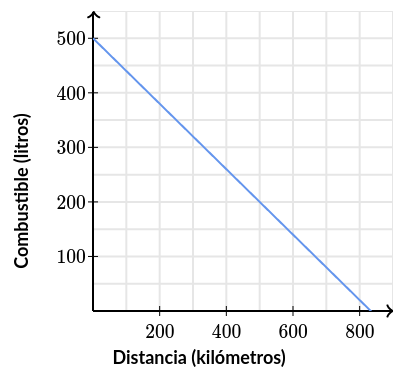
\includegraphics[width=0.7\linewidth]{../images/alaska_combustible}
            \caption{Gráfica de la cantidad de combustible que queda en el tanque del camión (en litros) como una función de la
                distancia que recorrió (en kilómetros)}
            \label{fig:alaska_combustible}
        \end{figure}

        \textbf{¿Cuánto combustible consume el tanque cada 100 kilómetros?}

        \begin{oneparchoices}
            \CorrectChoice 60 L
            \choice 0.5 L
            \choice 500 L
            \choice 0.6 L
        \end{oneparchoices}

        \part  Harry obtuvo un préstamo del banco.
        La variable $D$ modela la deuda restante de Harry (en pesos) como función del tiempo $t$ en meses desde que obtuvo el préstamo.
        \[D=-200t+9000\]
        \textbf{¿Cuánto dinero paga Harry cada mes?}

        \$\fillin[200][1cm]

        \part Andrei quiere llenar un tanque de vidrio con canicas, y luego el espacio restante con agua.
        La variable $w$ modela la cantidad de agua (en litros) que Andrei usa si utiliza $n$ canicas.
        \[w=32-0.05n\]
        \textbf{¿Cuál es el volumen de cada canica?}

        \fillin[0.05][1cm] litros.

        \part La temperatura puede medirse en dos unidades comunes: grados Celsius y grados Fahrenheit.
        La variable $F$ representa la temperatura en grados Fahrenheit que es equivalente a la temperatura $C$ en grados Celsius.
        \[F=32+1.8C\]
        \textbf{¿Cuál es el incremento en grados Fahrenheit equivalente a un incremento de 10 grados Celsius?}

        \fillin[18][1cm] grados Fahrenheit.

    \end{parts}
\end{multicols}
